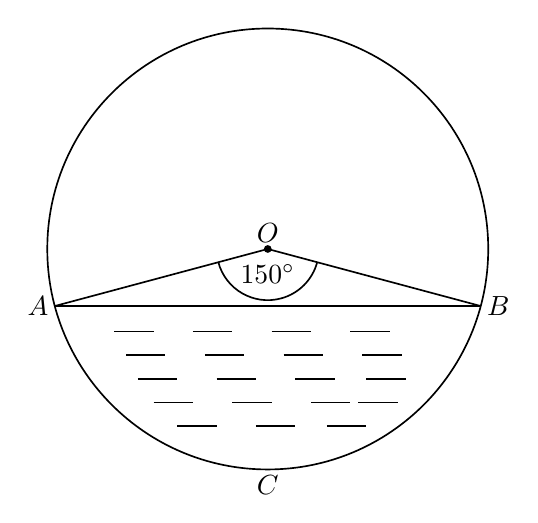
\begin{tikzpicture}[x=1cm,y=1cm,line width=.6pt,font=\normalsize,water dash/.style={draw=black,line width=.6pt}]
\coordinate (O) at (0,0);
\coordinate (A) at (-2.70459,-0.72469);
\coordinate (B) at (2.70459,-0.72469);
\coordinate (C) at (0,-2.8);
\coordinate (ANGLE) at (0,-0.32);
\coordinate (ARCS) at (-0.62785,-0.16823);
\coordinate (ARCE) at (0.62785,-0.16823);
\draw (O) circle[radius=2.8cm];
\draw (O)--(A);
\draw (O)--(B);
\draw (A)--(B);
\draw (ARCS) arc[start angle=195,end angle=345,radius=0.65cm];
\draw[water dash] (-1.95,-1.05)--(-1.45,-1.05);
\draw[water dash] (-0.95,-1.05)--(-0.45,-1.05);
\draw[water dash] (0.05,-1.05)--(0.55,-1.05);
\draw[water dash] (1.05,-1.05)--(1.55,-1.05);
\draw[water dash] (-1.80,-1.35)--(-1.30,-1.35);
\draw[water dash] (-0.80,-1.35)--(-0.30,-1.35);
\draw[water dash] (0.20,-1.35)--(0.70,-1.35);
\draw[water dash] (1.20,-1.35)--(1.70,-1.35);
\draw[water dash] (-1.65,-1.65)--(-1.15,-1.65);
\draw[water dash] (-0.65,-1.65)--(-0.15,-1.65);
\draw[water dash] (0.35,-1.65)--(0.85,-1.65);
\draw[water dash] (1.25,-1.65)--(1.75,-1.65);
\draw[water dash] (-1.45,-1.95)--(-0.95,-1.95);
\draw[water dash] (-0.45,-1.95)--(0.05,-1.95);
\draw[water dash] (0.55,-1.95)--(1.05,-1.95);
\draw[water dash] (1.15,-1.95)--(1.65,-1.95);
\draw[water dash] (-1.15,-2.25)--(-0.65,-2.25);
\draw[water dash] (-0.15,-2.25)--(0.35,-2.25);
\draw[water dash] (0.75,-2.25)--(1.25,-2.25);
\node[left=2pt,inner sep=0pt] at (A) {$A$};
\node[right=2pt,inner sep=0pt] at (B) {$B$};
\node[above=2pt,inner sep=0pt] at (O) {$O$};
\node[below=2pt,inner sep=0pt] at (C) {$C$};
\node at (ANGLE) {$150^{\circ}$};

% Explicit named circle-center points, painted after all region fills.
\fill (O) circle[radius=1.4pt];
\end{tikzpicture}
